FALTA LO DE ARRIBA EN PAGINA 19

\part{El canal discreto con ruido}
\label{part:2}

\chapter{Representaci\'{o}n de un canal discreto con ruido}
\label{sec:11}

FALTA

\clearpage

\chapter{Equivocaci\'{o}n y capacidad de canal}
\label{sec:12}

FALTA

\begin{theorem}
\label{th:10}
Si el canal de correcci\'{o}n...
\end{theorem}

FALTA

\begin{figure}[!ht]
\centerline{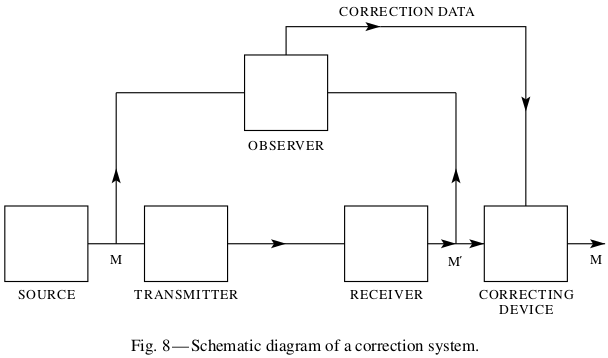
\includegraphics[width=120mm]{Imagenes/Pagina21-Figura8.png}}
\caption{Un diagrama esquem\'{a}tico de un sistema de correcci\'{o}n.}
\label{fig:8}
\end{figure}

FALTA

\begin{exmp}
Suponga que los errores suceden al azar...
\end{exmp}

FALTA

\begin{theorem}
\label{th:11}
Que un canal discreto tenga
\end{theorem}

FALTA

\clearpage

\chapter{El teorema fundamental para un canal discreto con ruido}
\label{sec:13}

\begin{figure}[!ht]
\centerline{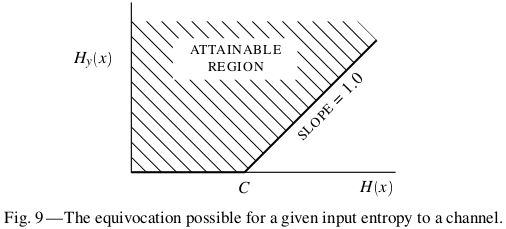
\includegraphics[width=100mm]{Imagenes/Pagina22-Figura9.png}}
\caption{La equivocaci\'{o}n posible para una entropia de entrada dada
  a un canal.}
\label{fig:9}
\end{figure}

FALTA

\begin{figure}[!ht]
\centerline{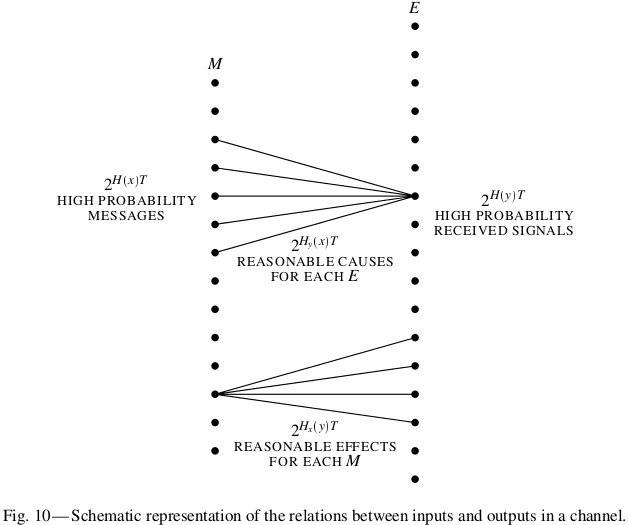
\includegraphics[width=140mm]{Imagenes/Pagina23-Figura10.png}}
\caption{Una representaci\'{o}n esquem\'{a}tica de las relaciones
  entre las entradas y salidas en un canal.}
\label{fig:10}
\end{figure}

FALTA

\clearpage

\chapter{Discussion}
\label{sec:14}

FALTA

